\documentclass{article}

% --- PRÉAMBULE ---
\usepackage[utf8]{inputenc}
\usepackage[T1]{fontenc}
\usepackage[numbers]{natbib}
\usepackage[french]{babel}
\usepackage{amsmath, amssymb}
\usepackage{geometry}
\usepackage{graphicx}
\usepackage{booktabs}
\usepackage{enumitem}
\usepackage{nicefrac}
\usepackage{tabularx}
\usepackage{longtable}
\usepackage{float}
\usepackage{xcolor}
\usepackage{colortbl}
\usepackage{listings}
\usepackage[protrusion=true,expansion=false]{microtype}

\usepackage{hyperref}
\hypersetup{
    colorlinks=true,
    linkcolor=blue,
    urlcolor=blue,
    citecolor=red,
    pdfborder={0 0 0}
}

\geometry{a4paper, margin=2.5cm}

\usepackage{tikz}
\usetikzlibrary{positioning, arrows.meta, shapes.geometric, calc,
                shapes.multipart}

% --- Couleurs ---
\definecolor{dbblue}{RGB}{10, 22, 40}
\definecolor{lightgray}{RGB}{245, 246, 248}
\definecolor{codegray}{RGB}{248, 248, 248}
\definecolor{sqlkw}{RGB}{0, 0, 180}

% --- Listings SQL / Python ---
\lstdefinestyle{sql}{
  language=SQL,
  basicstyle=\ttfamily\footnotesize,
  keywordstyle=\color{sqlkw}\bfseries,
  commentstyle=\color{gray}\itshape,
  backgroundcolor=\color{codegray},
  frame=single, rulecolor=\color{gray!40},
  numbers=left, numberstyle=\tiny\color{gray},
  breaklines=true, keepspaces=true,
}
\lstdefinestyle{python}{
  language=Python,
  basicstyle=\ttfamily\footnotesize,
  keywordstyle=\color{sqlkw}\bfseries,
  commentstyle=\color{gray}\itshape,
  backgroundcolor=\color{codegray},
  frame=single, rulecolor=\color{gray!40},
  numbers=left, numberstyle=\tiny\color{gray},
  breaklines=true, keepspaces=true,
}

% --- Styles TikZ (MCD) ---
\tikzset{
  entity/.style={
    draw=dbblue, line width=0.8pt,
    rectangle split, rectangle split parts=2,
    rectangle split part fill={dbblue, white},
    rectangle split part align={center, left},
    text width=3.4cm, font=\scriptsize,
    inner sep=3pt,
  },
  entity sm/.style={
    draw=dbblue, line width=0.8pt,
    rectangle split, rectangle split parts=2,
    rectangle split part fill={dbblue, white},
    rectangle split part align={center, left},
    text width=2.9cm, font=\scriptsize,
    inner sep=2pt,
  },
  rel/.style={draw=black!55, line width=0.7pt},
  relD/.style={draw=black!55, line width=0.7pt, dashed},
  card/.style={font=\tiny\bfseries, fill=white, inner sep=1.5pt},
}

\newcommand{\eh}[1]{\textcolor{white}{\normalfont\bfseries\footnotesize #1}}
\newcommand{\ea}[1]{\textcolor{black}{\scriptsize #1}}

% --- Titre ---
\title{\textbf{Rapport Technique}\\[0.4em]
       \large HealthAI Coach — Projet Data Engineering\\[0.2em]
       \normalsize Simplon Formation Data Engineer}
\author{Alexandre Laugier\thanks{Rôle A — Architecte / Lead Data Engineer : schéma base de données, interface admin (Gradio), dashboard Metabase, dockerisation}
        \and Florian Abgrall\thanks{Rôle B — API REST (FastAPI)}
        \and Johane Decamps\thanks{Rôle C — ETL (extract/transform/load), orchestration Airflow} \and William Mibelli\thanks{Rôle C — ETL (extract/transform/load), orchestration Airflow}}
\date{Juillet 2026}

% =============================================================================
\begin{document}
% =============================================================================

\sloppy

\maketitle
\thispagestyle{plain}
\newpage

\tableofcontents
\newpage

% =============================================================================
\section{Introduction}
% =============================================================================

HealthAI Coach est une plateforme de coaching santé : suivi nutritionnel, suivi de l'activité physique, relevés biométriques et profil médical déclaratif d'un utilisateur, avec génération de recommandations personnalisées (diététiques, puis plans d'entraînement/nutrition via un microservice IA à venir). Ce dépôt couvre exclusivement le \textbf{backend data} du projet : modélisation et administration de la base de données, pipeline ETL d'ingestion depuis des sources hétérogènes (Kaggle, API publique d'exercices), API REST, supervision de la qualité des données, et conteneurisation de l'ensemble — pas le frontend utilisateur final, hors périmètre de cette formation.

Le modèle économique conditionne plusieurs choix techniques documentés dans ce rapport : offre freemium (\texttt{free}/\texttt{premium}/\texttt{premium\_plus}) avec fonctionnalités IA réservées aux paliers payants, et offre B2B en marque blanche pour des organisations partenaires (salles de sport, mutuelles, entreprises), provisionnée par un administrateur plutôt qu'en self-service.

Travail réparti en trois rôles : Rôle A — architecture, base de données, interface admin (qualité des données), dashboard Metabase et dockerisation (Alexandre Laugier) ; Rôle B — API REST FastAPI (Florian Abgrall) ; Rôle C — pipeline ETL et orchestration Airflow (Johane Decamps, William Mibelli). Le développement suit un flux Pull Request systématique (une étape = une PR, tests obligatoires, revue avant fusion) détaillé dans \texttt{docs/plan\_de\_developpement.md}.

% =============================================================================
\section{Architecture du système}
% =============================================================================

\subsection{Vue d'ensemble}

\begin{figure}[H]
\centering
\resizebox{0.85\textwidth}{!}{%
\begin{tikzpicture}[node distance=1cm and 1.6cm, >=Stealth, box/.style={draw=dbblue, line width=0.8pt, rounded corners=2pt, fill=dbblue!6, minimum height=1.1cm, minimum width=2.6cm, align=center, font=\footnotesize}]

\node[box] (kaggle) {Sources externes\\\scriptsize Kaggle, API ExerciseDB};
\node[box, right=of kaggle] (etl) {ETL\\\scriptsize extract / transform / load};
\node[box, above=0.6cm of etl] (airflow) {Airflow\\\scriptsize orchestration, DAG};
\node[box, right=of etl] (pg) {PostgreSQL\\\scriptsize 16 tables};
\node[box, above right=0.3cm and 1.4cm of pg] (api) {API REST\\\scriptsize FastAPI};
\node[box, below right=0.3cm and 1.4cm of pg] (admin) {Interface admin\\\scriptsize Gradio};
\node[box, right=2.6cm of admin] (metabase) {Metabase\\\scriptsize dashboard KPI};

\draw[rel, ->] (kaggle) -- (etl);
\draw[rel, ->] (airflow) -- (etl);
\draw[rel, ->] (etl) -- (pg);
\draw[rel, ->] (pg) -- (api);
\draw[rel, ->] (pg) -- (admin);
\draw[rel, ->] (pg) -- (metabase);

\end{tikzpicture}}
\caption{Vue d'ensemble — l'ETL alimente PostgreSQL (orchestré par Airflow), consommé en aval par l'API REST, l'interface admin et Metabase. L'ensemble du périmètre est conteneurisé via \texttt{docker compose} (cf. \S\ref{sec:docker}).}
\label{fig:archi}
\end{figure}

\subsection{Choix technologiques}

\begin{table}[H]
\centering
\small
\begin{tabular}{@{}ll@{}}
\toprule
\textbf{Composant} & \textbf{Technologie} \\
\midrule
Base de données & PostgreSQL \\
Migrations & Alembic \\
Orchestration & Apache Airflow \\
API & FastAPI (SQLAlchemy, Pydantic, JWT) \\
Dashboard & Metabase \\
Interface admin & Gradio \\
Conteneurisation & Docker / Docker Compose \\
CI & GitHub Actions \\
\bottomrule
\end{tabular}
\caption{Stack technique (\texttt{README.md}).}
\end{table}

Deux choix méritent d'être justifiés au-delà du tableau : \textbf{PostgreSQL}~\citep{postgresql} plutôt qu'un SGBD NoSQL, parce que le domaine (utilisateurs, journaux nutrition/exercice historisés, contraintes d'intégrité inter-tables) est structurellement relationnel — les nombreuses contraintes \texttt{CHECK}/\texttt{FOREIGN KEY} qui portent une partie significative des règles métier (cf. \S3.2) auraient dû être réimplémentées côté application dans un magasin sans schéma. \textbf{Gradio}~\citep{gradio} plutôt qu'un framework front complet (React, Streamlit) pour l'interface admin, parce qu'il s'agit d'un outil interne à faible surface (un seul écran, quelques formulaires) où la rapidité de mise en œuvre prime sur la personnalisation visuelle — au prix de limitations d'accessibilité propres au composant \texttt{Dataframe}, documentées en \S\ref{sec:admin-interface}.

% =============================================================================
\section{Modélisation des données}
% =============================================================================

Le schéma relationnel (\texttt{database/schema/ddl\_postgres.sql}) compte 16 tables, réparties en cinq domaines fonctionnels autour de l'entité centrale \texttt{USERS} : nutrition, activité physique, suivi déclaratif de santé, abonnements, et contenu généré par IA. Chaque table porte des commentaires SQL (\texttt{COMMENT ON TABLE/COLUMN}) documentant directement en base la signification de chaque champ — en particulier les conventions non triviales comme les clés d'idempotence \texttt{UNIQUE(source, external\_id)}.

\subsection{Modèle Conceptuel de Données — périmètre OLTP}

La figure~\ref{fig:mcd-core} présente le cœur du modèle : nutrition, activité physique, suivi de santé déclaratif et contenu généré par IA (\texttt{workout\_plans}/\texttt{nutrition\_plans}), tous rattachés à \texttt{USERS}. La figure~\ref{fig:mcd-subscriptions} présente le domaine abonnements, ajouté dans un second temps pour l'offre B2C/B2B.

\begin{figure}[H]
\centering
\resizebox{\textwidth}{!}{%
\begin{tikzpicture}[node distance=1.1cm and 1.1cm, >=Stealth]

\node[entity] (food) {\eh{FOOD\_ITEMS}
\nodepart{two}\ea{food\_item\_id (PK)\\source, external\_id (UK)\\name, calories\_kcal...}};

\node[entity, below=of food] (nutlog) {\eh{NUTRITION\_\\LOGS}
\nodepart{two}\ea{log\_id (PK)\\user\_id (FK)\\food\_item\_id (FK)\\portion\_number, meal\_type}};

\node[entity, right=6.4cm of food] (exo) {\eh{EXERCISES}
\nodepart{two}\ea{exercise\_id (PK)\\source, external\_id (UK)\\name, body\_part...}};

\node[entity, below=of exo] (sets) {\eh{WORKOUT\_\\SETS}
\nodepart{two}\ea{set\_id (PK)\\session\_id (FK)\\exercise\_id (FK)\\reps, weight\_kg...}};

\node[entity, below=of sets] (sess) {\eh{WORKOUT\_\\SESSIONS}
\nodepart{two}\ea{session\_id (PK)\\user\_id (FK)\\started\_at, ended\_at\\max\_bpm, avg\_bpm}};

\node[entity, below right=2.9cm and -0.3cm of nutlog] (users) {\eh{USERS}
\nodepart{two}\ea{user\_id (PK)\\email (UK), sex\\is\_admin}};

\node[entity sm, below=3.6cm of users] (bio) {\eh{BIOMETRIC\_\\MEASUREMENTS}
\nodepart{two}\ea{measurement\_id (PK)\\user\_id (FK)\\weight\_kg, height\_cm...}};

\node[entity sm, left=0.5cm of bio] (med) {\eh{MEDICAL\_\\PROFILES}
\nodepart{two}\ea{medical\_profile\_id (PK)\\user\_id (FK)\\disease\_type, severity...}};

\node[entity sm, left=0.5cm of med] (dql) {\eh{DATA\_QUALITY\_\\LOG}
\nodepart{two}\ea{dq\_log\_id (PK)\\source\_table\\resolved\_by (FK, optionnelle)}};

\node[entity sm, right=0.5cm of bio] (diet) {\eh{DIETARY\_\\PREFERENCES}
\nodepart{two}\ea{dietary\_preference\_id (PK)\\user\_id (FK)\\allergies...}};

\node[entity sm, right=0.5cm of diet] (fit) {\eh{FITNESS\_\\PROFILES}
\nodepart{two}\ea{fitness\_profile\_id (PK)\\user\_id (FK)\\experience\_level...}};

\node[entity sm, right=0.5cm of fit] (rec) {\eh{DIET\_\\RECOMMEN\-DATIONS}
\nodepart{two}\ea{diet\_recommendation\_id (PK)\\user\_id (FK)\\recommendation...}};

\node[entity sm, right=0.5cm of rec] (wplan) {\eh{WORKOUT\_\\PLANS}
\nodepart{two}\ea{workout\_plan\_id (PK)\\user\_id (FK)\\goal, plan\_text...}};

\node[entity sm, right=0.5cm of wplan] (nplan) {\eh{NUTRITION\_\\PLANS}
\nodepart{two}\ea{nutrition\_plan\_id (PK)\\user\_id (FK)\\goal, plan\_text...}};

% Relations — cardinalités Merise (min,max), lues côté entité adjacente
\draw[rel] (food) -- (nutlog) node[card, pos=0.15]{(0,N)} node[card, pos=0.85]{(1,1)};
\draw[rel] (nutlog.east) -- ++(0.6,0) |- (users.north west) node[card, pos=0.05]{(1,1)} node[card, pos=0.78, xshift=-2pt, yshift=6pt]{(0,N)};
\draw[rel] (exo) -- (sets) node[card, pos=0.15]{(0,N)} node[card, pos=0.85]{(1,1)};
\draw[rel] (sets) -- (sess) node[card, pos=0.15]{(1,1)} node[card, pos=0.85]{(0,N)};
\draw[rel] (sess.west) -- ++(-0.6,0) |- (users.north east) node[card, pos=0.05]{(1,1)} node[card, pos=0.78, xshift=2pt, yshift=6pt]{(0,N)};

% Points d'ancrage répartis le long du bord sud de USERS — évite que les
% 8 connexions vers la rangée du bas ne partent toutes du même point.
\coordinate (u1) at ($(users.south west)!0.04!(users.south east)$);
\coordinate (u2) at ($(users.south west)!0.17!(users.south east)$);
\coordinate (u3) at ($(users.south west)!0.30!(users.south east)$);
\coordinate (u4) at ($(users.south west)!0.43!(users.south east)$);
\coordinate (u5) at ($(users.south west)!0.57!(users.south east)$);
\coordinate (u6) at ($(users.south west)!0.70!(users.south east)$);
\coordinate (u7) at ($(users.south west)!0.83!(users.south east)$);
\coordinate (u8) at ($(users.south west)!0.96!(users.south east)$);

\draw[relD] (u1) -- (dql.north) node[card, pos=0.30]{(0,N)} node[card, pos=0.88]{(0,1)};
\draw[rel] (u2) -- (med.north) node[card, pos=0.28]{(0,N)} node[card, pos=0.88]{(1,1)};
\draw[rel] (u3) -- (bio.north) node[card, pos=0.26]{(0,N)} node[card, pos=0.88]{(1,1)};
\draw[rel] (u4) -- (diet.north) node[card, pos=0.24]{(0,N)} node[card, pos=0.88]{(1,1)};
\draw[rel] (u5) -- (fit.north) node[card, pos=0.24]{(0,N)} node[card, pos=0.88]{(1,1)};
\draw[rel] (u6) -- (rec.north) node[card, pos=0.26]{(0,N)} node[card, pos=0.88]{(1,1)};
\draw[rel] (u7) -- (wplan.north) node[card, pos=0.28]{(0,N)} node[card, pos=0.88]{(1,1)};
\draw[rel] (u8) -- (nplan.north) node[card, pos=0.30]{(0,N)} node[card, pos=0.88]{(1,1)};

\end{tikzpicture}}

\vspace{0.2cm}
\noindent\tikz[baseline=-0.5ex]{\draw[rel] (0,0) -- (0.6,0);} FK obligatoire (\texttt{NOT NULL}) \hspace{2em}
\tikz[baseline=-0.5ex]{\draw[relD] (0,0) -- (0.6,0);} FK optionnelle (\texttt{NULL} autorisé)

\caption{MCD — cœur du modèle (nutrition, activité physique, suivi de santé, contenu IA). Cardinalités au format Merise (min,max), lues côté entité adjacente.}
\label{fig:mcd-core}
\end{figure}

\begin{figure}[H]
\centering
\resizebox{0.7\textwidth}{!}{%
\begin{tikzpicture}[node distance=1.6cm and 1.6cm, >=Stealth]

\node[entity] (org) {\eh{ORGANIZATIONS}
\nodepart{two}\ea{organization\_id (PK)\\name, contact\_email}};

\node[entity, right=of org] (sub) {\eh{SUBSCRIPTIONS}
\nodepart{two}\ea{subscription\_id (PK)\\user\_id (FK)\\organization\_id (FK, optionnelle)\\tier, status, price\_eur\_cents}};

\node[entity, right=of sub] (usr2) {\eh{USERS}
\nodepart{two}\ea{user\_id (PK)\\email (UK)}};

\draw[relD] (org) -- (sub) node[card, pos=0.15]{(0,N)} node[card, pos=0.85]{(0,1)};
\draw[rel] (sub) -- (usr2) node[card, pos=0.15]{(1,1)} node[card, pos=0.85]{(0,N)};

\end{tikzpicture}}

\vspace{0.2cm}
\noindent\tikz[baseline=-0.5ex]{\draw[rel] (0,0) -- (0.6,0);} FK obligatoire (\texttt{NOT NULL}) \hspace{2em}
\tikz[baseline=-0.5ex]{\draw[relD] (0,0) -- (0.6,0);} FK optionnelle (\texttt{NULL} autorisé)

\caption{MCD — domaine abonnements. \texttt{organization\_id} n'est renseigné que pour \texttt{tier = 'b2b'} (contrainte \texttt{chk\_subscriptions\_b2b\_organization}).}
\label{fig:mcd-subscriptions}
\end{figure}

\subsection{Contraintes d'intégrité et conventions}

Le schéma s'appuie sur PostgreSQL pour porter un maximum de règles métier directement en base plutôt que dans le code applicatif, avec quatre familles de contraintes récurrentes :

\begin{itemize}[leftmargin=1.4em]
  \item \textbf{Domaines de valeurs} — \texttt{CHECK} sur les colonnes à choix fermé : \texttt{sex IN ('F', 'M', 'other')}, \texttt{severity IN ('info', 'warning', 'error', 'critical')} (\texttt{data\_quality\_log}), \texttt{meal\_type IN ('breakfast', 'lunch', 'dinner', 'snack')}, \texttt{tier IN ('free', 'premium', 'premium\_plus', 'b2b')}. Ces contraintes ont capturé un bug réel en cours de développement : un mapping de valeurs dans l'ETL produisait \texttt{'Other'} (majuscule) au lieu de \texttt{'other'}, rejeté par PostgreSQL (\texttt{CheckViolation}) mais indétecté par les tests unitaires du module, qui mockaient la base — cf. \S\ref{sec:tests}.

  \item \textbf{Cohérence inter-colonnes} — \texttt{CHECK} portant sur plusieurs colonnes de la même ligne : \texttt{ended\_at >= started\_at} (\texttt{workout\_sessions}, \texttt{subscriptions}), ou la cohérence B2B \texttt{(tier = 'b2b' AND organization\_id IS NOT NULL) OR (tier <> 'b2b' AND organization\_id IS NULL)} qui garantit qu'une organisation n'est renseignée que pour les abonnements B2B, et inversement.

  \item \textbf{Idempotence au chargement} — \texttt{food\_items} et \texttt{exercises} portent \texttt{UNIQUE(source, external\_id)} : la paire (origine de la donnée, identifiant dans la source) sert de clé d'upsert (\texttt{INSERT ... ON CONFLICT DO UPDATE}) pour que les DAG Airflow puissent être rejoués sans dupliquer les données. Point de vigilance documenté et transmis à l'équipe ETL : \texttt{biometric\_measurements} porte \texttt{UNIQUE(user\_id, measured\_at)} et non \texttt{UNIQUE(user\_id, source)} — si le chargement fixe \texttt{measured\_at = now()} au moment de l'ingestion, chaque ré-exécution génère un nouveau relevé au lieu de mettre à jour l'existant.

  \item \textbf{Génération de données manquantes, sans casser l'idempotence} — les datasets sources n'ont pas de champ nom (\texttt{first\_name}/\texttt{last\_name}, \texttt{NOT NULL} en base). Convention retenue : \texttt{Faker}~\citep{faker} avec une seed déterministe par ligne source (\texttt{Faker.seed(hash(patient\_id))}), pas un tirage aléatoire à chaque exécution — sinon un même utilisateur changerait de nom à chaque ré-exécution du DAG, ce qui casse la logique d'idempotence par ailleurs garantie par les \texttt{UNIQUE(source, external\_id)}.
\end{itemize}

% =============================================================================
\section{Pipeline ETL}
% =============================================================================

\subsection{Structure du pipeline}

Le pipeline suit un découpage classique en trois étapes, une responsabilité par module sous \texttt{etl/} :

\begin{itemize}[leftmargin=1.4em]
  \item \texttt{extract/extract.py} — télécharge les quatre jeux de données Kaggle (nutrition, diet, gym-members, fitness-tracker) et interroge l'API publique \texttt{oss.exercisedb.dev} (pagination gérée, tolère un \texttt{429} en cours de pagination sans faire échouer tout le run) ; écrit les fichiers bruts sous \texttt{etl/data/}.
  \item \texttt{transform/} — un module par source (\texttt{clean\_nutrition.py}, \texttt{clean\_exercises.py}, \texttt{clean\_diet.py}, \texttt{clean\_users.py}), chacun responsable du renommage des colonnes vers le schéma cible, du typage, et du remplissage des colonnes obligatoires absentes de la source (cf. \S3.2, convention \texttt{Faker.seed()}).
  \item \texttt{load/postgres\_loader.py} — chargement idempotent, deux techniques selon la table : \texttt{food\_items}/\texttt{exercises} passent par une table de staging (\texttt{to\_sql}) puis un \texttt{INSERT ... SELECT ... ON CONFLICT DO UPDATE} depuis le staging (clé \texttt{UNIQUE(source, external\_id)}) ; \texttt{users} par un \texttt{INSERT ... ON CONFLICT (email) DO UPDATE ... RETURNING user\_id} direct, dont l'identifiant sert ensuite à insérer les tables dépendantes (\texttt{biometric\_measurements}, \texttt{workout\_sessions}, \texttt{medical\_profiles}, \texttt{dietary\_preferences}).
\end{itemize}

\texttt{extract} et \texttt{load} exposent chacun une fonction d'entrée (\texttt{run()}, \texttt{load\_data()}) plutôt que d'exécuter leur logique au chargement du module — nécessaire pour un usage sûr depuis Airflow, qui importe périodiquement les fichiers DAG pour les parser sans vouloir déclencher un téléchargement ou une connexion base à chaque fois.

L'orchestration (Sprint 3) est un DAG Airflow~\citep{airflow} unique, \texttt{healthai\_etl\_pipeline} (\texttt{extract} $\rightarrow$ \texttt{transform\_and\_load} $\rightarrow$ \texttt{quality\_check}), plutôt qu'un DAG par source comme envisagé initialement : le volume et le nombre de sources de ce projet ne justifient pas la complexité d'une orchestration plus fine. \texttt{transform} et \texttt{load} sont une seule tâche parce qu'ils s'exécutent déjà dans le même processus côté code, sans artefact intermédiaire sur disque — les séparer aurait forcé à faire transiter des DataFrames pandas par XCom, déconseillé par la documentation Airflow au-delà de très petits volumes. \texttt{quality\_check} exécute des règles réelles (tables vides, valeurs plausibles mais suspectes, complétude) et journalise dans \texttt{data\_quality\_log} — jusqu'ici rien n'écrivait de vraies anomalies dans cette table en dehors du seed de démonstration.

\paragraph{Isolation de dépendances.} Airflow 2.10.5 exige \texttt{SQLAlchemy<2.0} en interne, incompatible avec le \texttt{2.0.51} utilisé partout ailleurs dans le projet (installer les deux dans le même environnement Python casse le webserver/scheduler — confirmé par les avertissements \texttt{pip} avant correction). Les dépendances ETL sont donc installées dans un venv dédié à l'intérieur de l'image Airflow (\texttt{/opt/etl-venv}), et chaque tâche du DAG est un \texttt{BashOperator} qui invoque ce venv en sous-processus plutôt qu'un \texttt{PythonOperator} qui importerait \texttt{etl/} dans le process Airflow lui-même.

\begin{figure}[H]
\centering
\resizebox{\textwidth}{!}{%
\begin{tikzpicture}[node distance=0.9cm and 1.2cm, >=Stealth,
  box/.style={draw=dbblue, line width=0.8pt, rounded corners=2pt, fill=dbblue!6, minimum height=1.3cm, minimum width=3.1cm, align=center, font=\footnotesize},
  hub/.style={box, fill=dbblue!16}]

\node[box] (extract) {Extraction\\\scriptsize \texttt{extract/extract.py}\\\scriptsize Kaggle, API ExerciseDB};
\node[box, right=of extract] (transform) {Transformation\\\scriptsize \texttt{transform/clean\_*.py}\\\scriptsize renommage colonnes, typage};
\node[box, right=of transform] (normalize) {Normalisation\\\scriptsize valeurs manquantes (\texttt{Faker.seed()}), valeurs contrôlées (\texttt{source}, \texttt{sex})};
\node[box, right=of normalize] (load) {Chargement\\\scriptsize \texttt{load/postgres\_loader.py}\\\scriptsize upsert idempotent (staging + \texttt{ON CONFLICT})};
\node[hub, below=1.3cm of load] (pg) {PostgreSQL};
\node[hub, above=1.4cm of transform, xshift=1.75cm] (airflow) {Airflow\\\scriptsize DAG unique, \texttt{BashOperator} + venv isolé};
\node[box, below=1.3cm of extract, draw=red!50!black, fill=red!5] (dq) {\texttt{data\_quality\_log}\\\scriptsize DAG qualité (anomalies)};

\draw[rel, ->] (extract) -- (transform);
\draw[rel, ->] (transform) -- (normalize);
\draw[rel, ->] (normalize) -- (load);
\draw[rel, ->] (load) -- (pg);
\draw[rel, ->] (airflow) -- (transform.north);
\draw[rel, ->] (airflow) -- (normalize.north);
\draw[rel, ->] (airflow.west) -| (extract.north);
\draw[rel, ->] (airflow.east) -| (load.north);
\draw[rel, ->, relD] (normalize) -- (dq);

\end{tikzpicture}}
\caption{Flux ETL : extraction (téléchargement brut vers \texttt{etl/data/}), transformation (renommage/typage), normalisation (remplissage déterministe des colonnes obligatoires absentes de la source, contrôle des valeurs), chargement (upsert idempotent) — orchestré par le DAG Airflow unique \texttt{healthai\_etl\_pipeline}, avec journalisation des anomalies réelles dans \texttt{data\_quality\_log}.}
\label{fig:etl-flow}
\end{figure}

\subsection{Données sources}

\begin{table}[H]
\centering
\small
\begin{tabularx}{\textwidth}{@{}p{3.4cm} X l@{}}
\toprule
\textbf{Source} & \textbf{Alimente} & \textbf{Valeur \texttt{source}} \\
\midrule
Kaggle — Daily Food and Nutrition~\citep{kaggle_nutrition} & \texttt{food\_items} & \texttt{kaggle\_\allowbreak daily\_\allowbreak food\_\allowbreak nutrition} \\
Kaggle — Diet Recommendations~\citep{kaggle_diet} & \texttt{medical\_profiles}, \texttt{dietary\_preferences} & (pas de \texttt{source}) \\
Kaggle — Gym Members Exercise~\citep{kaggle_gym} & \texttt{users}, \texttt{biometric\_measurements}, \texttt{workout\_sessions} & \texttt{kaggle\_\allowbreak gym\_\allowbreak members} \\
Kaggle — Fitness Tracker~\citep{kaggle_fitness} & \texttt{users}, \texttt{biometric\_measurements}, \texttt{workout\_sessions} & \texttt{kaggle\_\allowbreak gym\_\allowbreak members} \\
API \texttt{oss.exercisedb.dev}~\citep{exercisedb} & \texttt{exercises} & \texttt{exercisedb} \\
\bottomrule
\end{tabularx}
\caption{Correspondance source $\rightarrow$ table(s) alimentée(s). La colonne \texttt{source} est la clé de traçabilité et, combinée à \texttt{external\_id}, la clé d'upsert idempotent pour \texttt{food\_items}/\texttt{exercises} (cf. \S3.2).}
\end{table}

Point de vigilance transverse, documenté dans \texttt{docs/plan\_de\_developpement.md} et vérifié par relecture croisée avant fusion des PR de l'équipe ETL : la valeur exacte de \texttt{source} doit correspondre caractère pour caractère à celle attendue par la clé d'upsert et par \texttt{database/seed/seed\_data.py} (référence de mapping colonnes $\rightarrow$ tables) — une divergence silencieuse (ex. \texttt{'kaggle\_food\_nutrition'} au lieu de \texttt{'kaggle\_daily\_food\_nutrition'}) romprait la déduplication sans lever d'erreur SQL, puisque \texttt{source} n'est contrainte par aucun \texttt{CHECK} de valeurs. Ce type d'erreur ne se détecte pas par les tests unitaires du module \texttt{transform} (entrées mockées, aucun accès à une vraie base) : seule une vérification contre le schéma réel ou contre \texttt{seed\_data.py} le révèle.

\subsection{Qualité des données}

\texttt{data\_quality\_log} centralise les anomalies détectées par l'ETL (Sprint 3, tâche \texttt{quality\_check} du DAG \texttt{healthai\_etl\_pipeline}, \texttt{etl/quality/checks.py}) : table source, ligne concernée le cas échéant, règle déclenchée, sévérité (\texttt{info}/\texttt{warning}/\texttt{error}/\texttt{critical}), message. Consultation, filtrage et résolution manuelle des anomalies via l'interface admin (Sprint 5, \S\ref{sec:admin-interface}). La contrainte \texttt{chk\_data\_quality\_log\_resolution\_consistency} garantit qu'une anomalie non résolue ne porte ni \texttt{resolved\_at} ni \texttt{resolved\_by} — cohérence vérifiée par test (\texttt{tests/data\_quality/test\_schema.py}).

% =============================================================================
\section{API REST}
% =============================================================================

\subsection{Structure}

FastAPI~\citep{fastapi} (\texttt{api/main.py}), toutes les routes préfixées \texttt{/api/v1}. Structure en couches, une responsabilité par dossier :

\begin{itemize}[leftmargin=1.4em]
  \item \texttt{routers/} — la couche HTTP : un routeur par ressource, déclare les endpoints, valide les entrées via les schémas Pydantic~\citep{pydantic}, délègue à \texttt{crud/}.
  \item \texttt{crud/} — accès base de données (requêtes SQLAlchemy~\citep{sqlalchemy}), indépendant de FastAPI, ce qui permet de le tester sans monter d'application HTTP.
  \item \texttt{models/} — les entités SQLAlchemy (ORM), une classe par table.
  \item \texttt{schemas/} — les modèles Pydantic de requête/réponse (\texttt{...Create}, \texttt{...Read}, \texttt{...Update}), séparés des \texttt{models/} pour ne jamais exposer directement une colonne sensible (ex. \texttt{hashed\_password}) par accident.
\end{itemize}

Authentification par JWT (OAuth2 password flow) : \texttt{POST /auth/login} renvoie un jeton, envoyé ensuite en \texttt{Authorization: Bearer <token>}. Trois dépendances FastAPI réutilisables (\texttt{api/core/deps.py}) portent le contrôle d'accès : \texttt{CurrentUser} (authentifié), \texttt{CurrentAdmin} (403 si \texttt{is\_admin} faux), \texttt{CurrentPremiumUser} (403 hors palier payant, cf. \S5.3) — déclarées une fois, réutilisées comme simple type d'argument dans la signature de chaque route protégée. Documentation interactive auto-générée : \texttt{/docs} (Swagger UI), \texttt{/redoc}.

\begin{figure}[H]
\centering
\resizebox{0.62\textwidth}{!}{%
\begin{tikzpicture}[node distance=0.9cm, >=Stealth,
  box/.style={draw=dbblue, line width=0.8pt, rounded corners=2pt, fill=dbblue!6, minimum height=1.1cm, minimum width=6cm, align=center, font=\footnotesize},
  hub/.style={box, fill=dbblue!16}]

\node[box] (client) {Client HTTP\\\scriptsize requête + \texttt{Authorization: Bearer <token>}};
\node[box, below=of client] (auth) {\texttt{CurrentUser} / \texttt{CurrentAdmin} / \texttt{CurrentPremiumUser}\\\scriptsize décode le JWT, vérifie le rôle — 401/403 si échec};
\node[box, below=of auth] (router) {\texttt{routers/}\\\scriptsize valide la requête via \texttt{schemas/} (Pydantic)};
\node[box, below=of router] (crud) {\texttt{crud/}\\\scriptsize requêtes SQLAlchemy, indépendant de FastAPI};
\node[hub, below=of crud] (models) {\texttt{models/} (ORM) $\rightarrow$ PostgreSQL};

\draw[rel, ->] (client) -- (auth);
\draw[rel, ->] (auth) -- (router);
\draw[rel, ->] (router) -- (crud);
\draw[rel, ->] (crud) -- (models);

\end{tikzpicture}}
\caption{API REST — flux d'une requête authentifiée : vérification d'accès avant tout traitement métier, puis séparation stricte HTTP (\texttt{routers/}) / accès données (\texttt{crud/}) / persistance (\texttt{models/}).}
\label{fig:api-archi}
\end{figure}

\subsection{Endpoints principaux}

\begin{itemize}[leftmargin=1.4em]
  \item \textbf{auth} — inscription, connexion (émission du JWT).
  \item \textbf{users} / \textbf{admin} — profil de l'utilisateur authentifié ; gestion de tout compte, réservée aux admins.
  \item \textbf{food-items} / \textbf{exercises} — catalogues alimentés par l'ETL, lecture libre, écriture admin uniquement.
  \item \textbf{nutrition-logs} / \textbf{workouts} / \textbf{biometrics} / \textbf{health-profiles} — données propres à l'utilisateur authentifié (repas journalisés ; séances et séries d'entraînement ; relevés biométriques ; profils médical/alimentaire/de forme historisés et recommandations diététiques en lecture seule).
  \item \textbf{data-quality} — vue admin sur \texttt{data\_quality\_log} (cf. \S4.3) et résolution des anomalies, alternative programmatique à l'interface Gradio.
  \item \textbf{subscriptions} / \textbf{organizations} — auto-gestion de l'abonnement ; provisionnement B2B et gestion des organisations partenaires, admin uniquement (cf. \S5.3).
  \item \textbf{ai} — génération de contenu (recommandations, plans), réservée aux paliers payants (cf. \S5.3).
  \item \textbf{health} — \textit{liveness check} pour la supervision.
\end{itemize}

\subsection{Abonnements et microservices IA}

Quatre paliers (\texttt{subscriptions.tier}) : \texttt{free} (par défaut à l'inscription), \texttt{premium}, \texttt{premium\_plus}, et \texttt{b2b} (rattaché à une \texttt{organization}, provisionné par un admin — pas de self-service pour ce palier). Une seule souscription \texttt{active} à la fois par utilisateur (index unique partiel), changement de palier = clôture de l'ancienne + ouverture d'une nouvelle.

Le contenu IA (\texttt{POST /ai/diet-recommendations}, \texttt{/ai/workout-plans}, \texttt{/ai/nutrition-plans}) est réservé aux paliers payants via une dépendance dédiée (\texttt{CurrentPremiumUser}, \texttt{api/core/deps.py}) : 403 pour un compte \texttt{free}, 401 sans authentification. Le microservice IA lui-même n'est pas encore déployé (cf. issue \#49) : les routes et le stockage (tables \texttt{workout\_plans}, \texttt{nutrition\_plans}, plus le \texttt{diet\_recommendations} existant) sont préparés à l'avance, avec un client stub (\texttt{api/services/ai\_client.py}) reproduisant la signature du futur appel HTTP réel. Objectif : brancher le vrai microservice n'impliquera de changer que ce fichier, ni les routers ni le contrat \texttt{POST /ai/...} exposé aux clients. Vérifié par 136 tests réels contre PostgreSQL (gating par palier, persistance, isolation des données par utilisateur), cf. \S\ref{sec:tests}.

% =============================================================================
\section{Interface admin (Gradio) et dashboard Metabase}
\label{sec:admin-interface}
% =============================================================================

\subsection{Interface admin}

Outil interne (Sprint 5, \texttt{admin\_interface/app\_gradio.py}, thème \texttt{Gradio Soft}) destiné aux administrateurs (\texttt{users.is\_admin}) pour traiter les anomalies journalisées dans \texttt{data\_quality\_log} sans accès direct à la base :

\begin{itemize}[leftmargin=1.4em]
  \item \textbf{Consultation} — tableau filtrable par sévérité, statut de résolution et table source (filtre partiel), rafraîchi à la demande.
  \item \textbf{Correction manuelle} — résolution d'une anomalie par son \texttt{dq\_log\_id}, avec traçabilité optionnelle de l'administrateur ayant traité le cas (\texttt{resolved\_by}).
  \item \textbf{Export} — CSV et JSON du résultat filtré courant, dates sérialisées au format ISO.
\end{itemize}

Testé par 26 tests (\texttt{tests/admin\_interface/}) : logique pure (formatage, traduction des filtres) sans dépendance, et logique base de données sur un PostgreSQL jetable (cf. \S\ref{sec:tests}).

\begin{figure}[H]
\centering
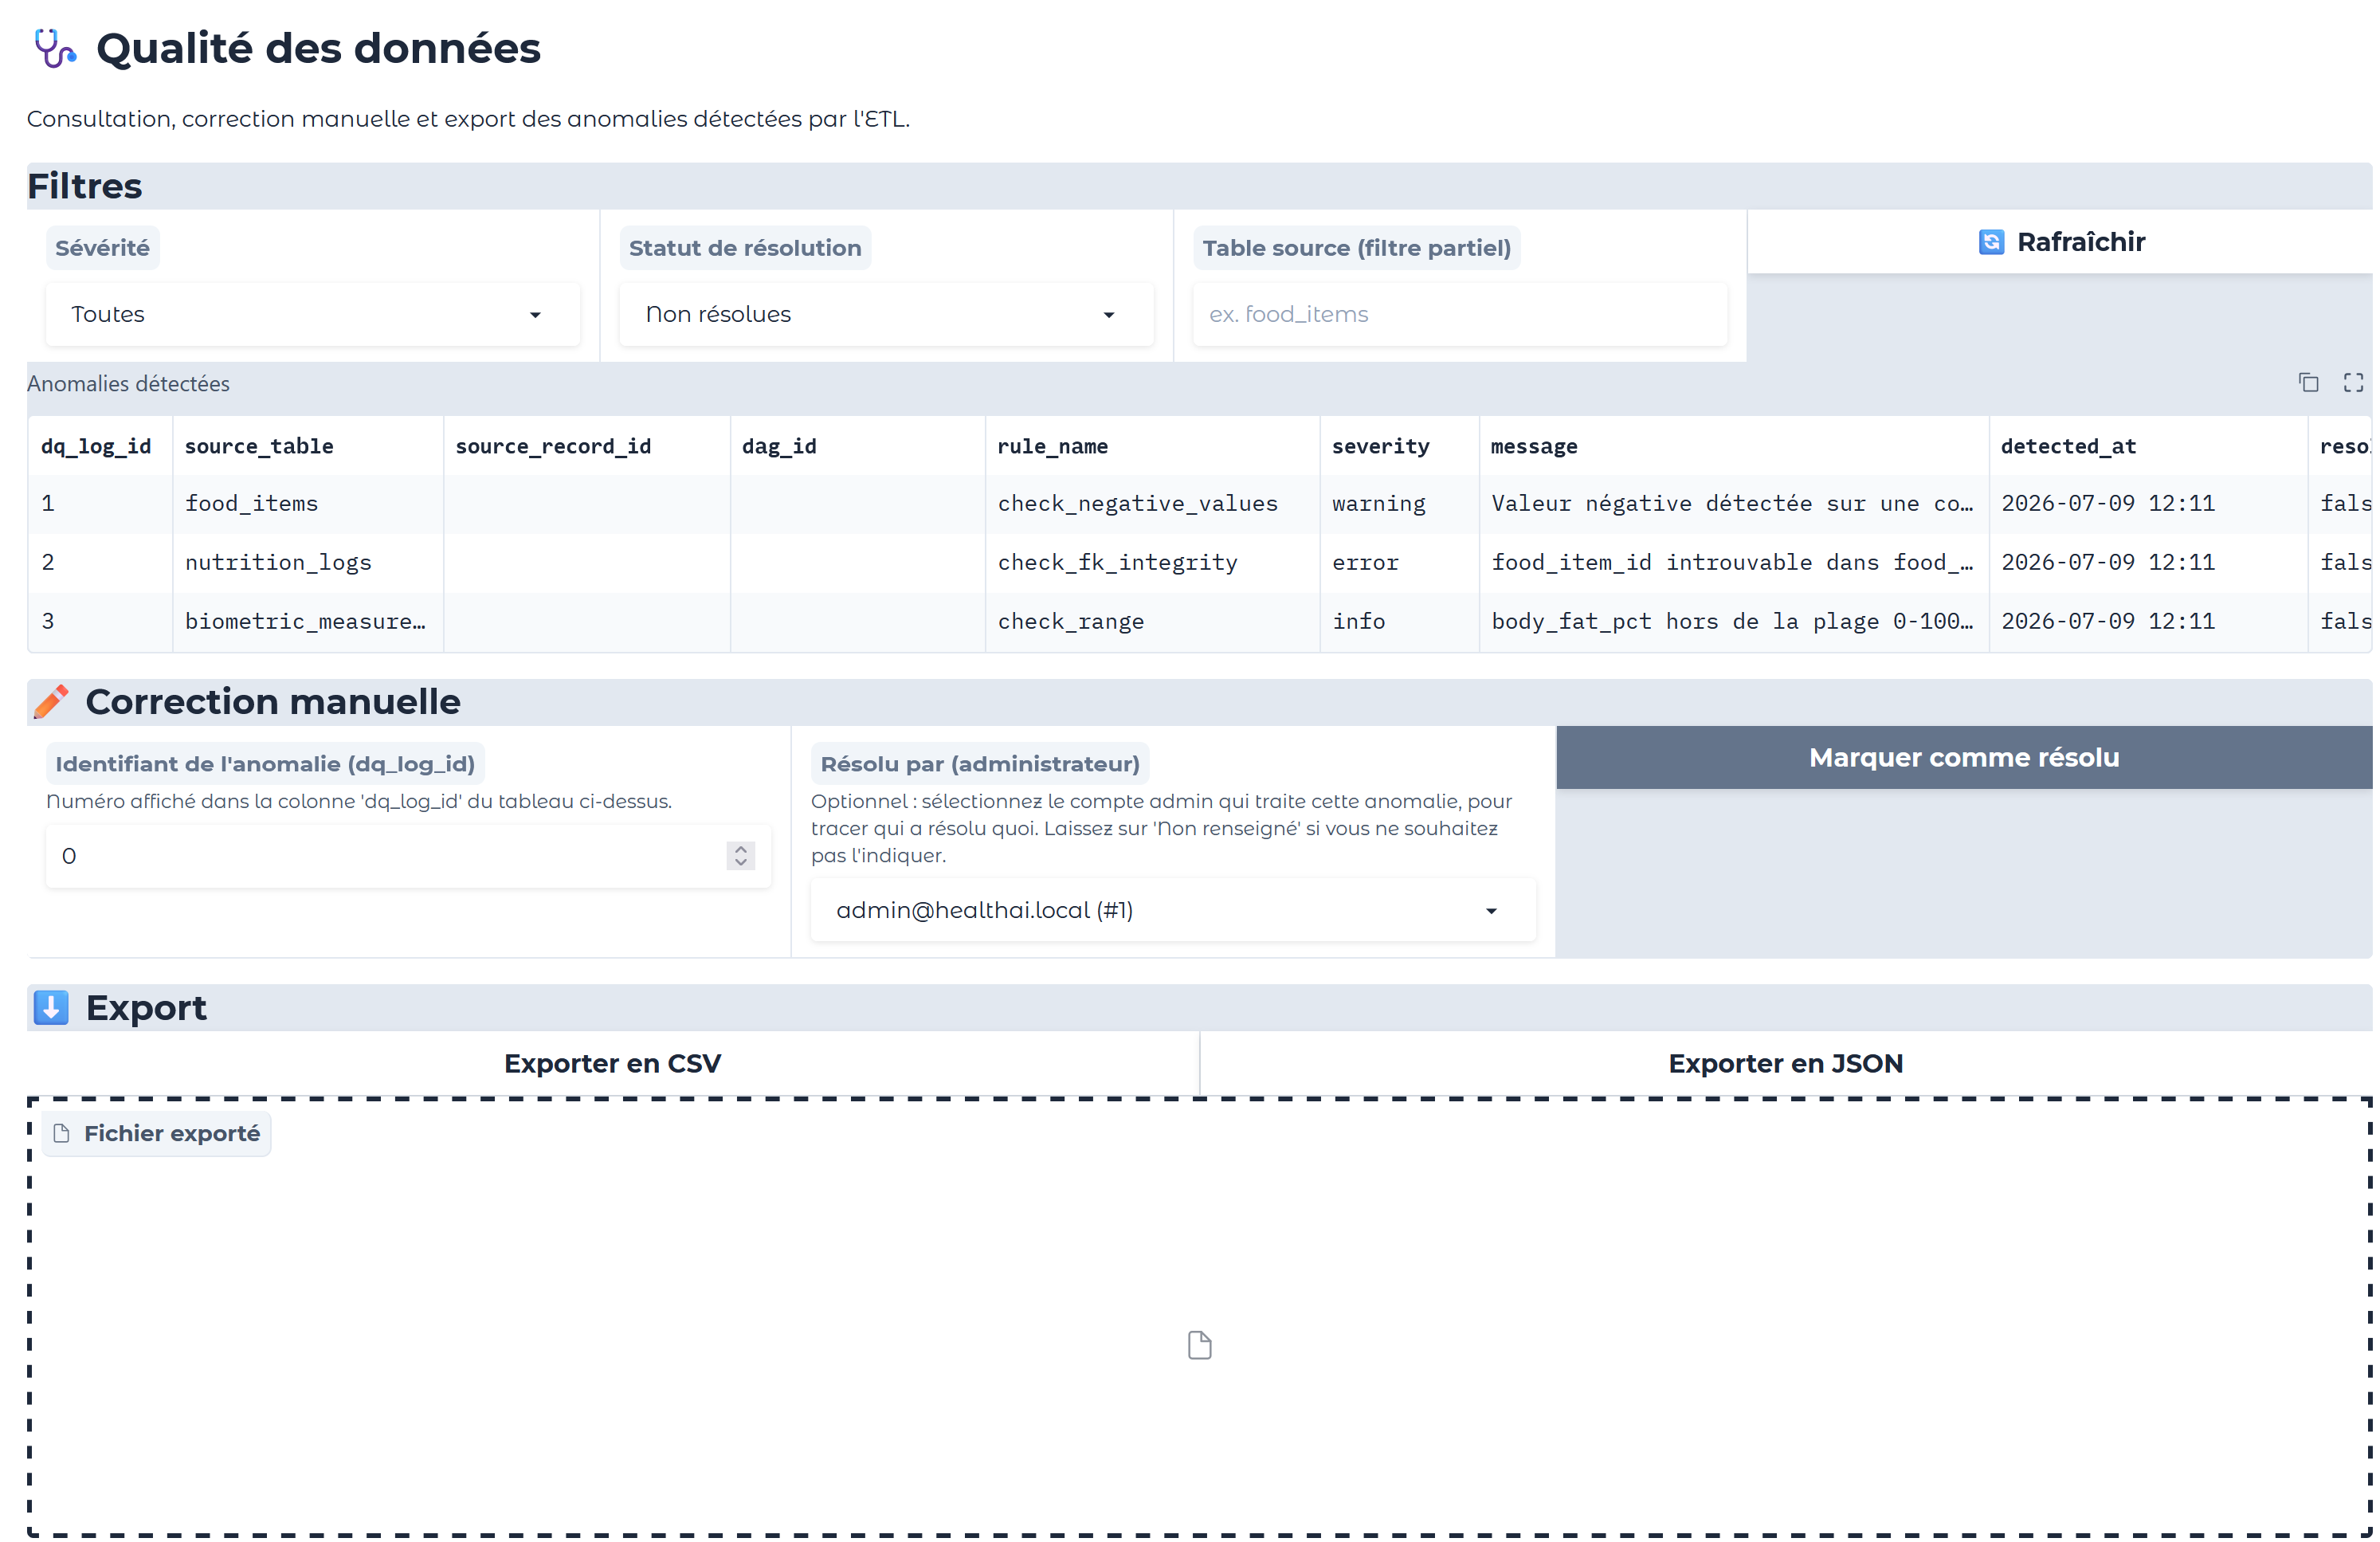
\includegraphics[width=\textwidth]{img/admin_interface_consultation.png}
\caption{Interface admin — filtres, consultation des anomalies, correction manuelle et export sur une même page.}
\label{fig:admin-interface}
\end{figure}

\subsection{Accessibilité RGAA}

Un audit automatisé (\texttt{axe-core}~\citep{axecore}, navigateur headless) a été mené sur l'interface plutôt qu'une simple relecture visuelle, pour objectiver le niveau de conformité RGAA~\citep{rgaa}/WCAG AA réellement atteint. Résultat, deux catégories distinctes :

\textbf{Corrigé, propre au code applicatif} —
\begin{itemize}[leftmargin=1.4em]
  \item \textit{Contraste insuffisant} : les couleurs de texte par défaut du thème \texttt{Soft} échouaient au seuil AA de 4,5:1 — labels de champs à 4,34:1, texte d'aide (\texttt{info=}) à 2,56:1 (échec net). Cause : \texttt{block\_label\_text\_color} et \texttt{block\_info\_text\_color} valent respectivement \texttt{*neutral\_500}/\texttt{*neutral\_400} par défaut dans Gradio. Corrigé en les fixant explicitement à \texttt{*neutral\_600} (\texttt{\#475569}), ce qui porte le ratio à 6,1--7,6:1 selon le fond concerné (vérifié par calcul de luminance relative sur les trois fonds rencontrés : blanc, \texttt{\#f1f5f9}, \texttt{\#e2e8f0}).
  \item \textit{Hiérarchie de titres invalide} : le titre principal (\texttt{h1}) était suivi directement de sous-titres en \texttt{h3} (\texttt{Filtres}, \texttt{Correction manuelle}, \texttt{Export}), sans niveau \texttt{h2} intermédiaire. Corrigé en repassant ces sous-titres en \texttt{h2}.
\end{itemize}

\textbf{Non corrigible depuis le code applicatif} — le composant \texttt{Dataframe} de Gradio génère, pour son mécanisme de glisser-déposer CSV/TSV, un bouton englobant l'ensemble des cellules et en-têtes du tableau (chacun rendu comme \texttt{span role="button"} individuellement focusable), ce qui viole plusieurs règles ARIA : éléments interactifs imbriqués (\texttt{nested-interactive}), noms accessibles manquants sur les cellules (\texttt{aria-command-name}), structure de grille invalide (\texttt{aria-required-children}). Confirmé indépendamment par un test de navigation clavier (parcours \texttt{Tab} sur 8 arrêts) : le tableau se comporte comme un unique arrêt de focus englobant, sans granularité cellule par cellule utilisable au clavier/lecteur d'écran. Ces défauts sont internes au rendu du composant Gradio, documentés comme limitation connue plutôt que contournés (un contournement aurait nécessité de reconstruire le composant tableau, hors de portée du calendrier).

\subsection{Dashboard Metabase}

Instance self-hosted de Metabase~\citep{metabase} (\texttt{docker compose}, cf. \S7), connectée en lecture à PostgreSQL. Au-delà des 14 tables du schéma, plusieurs vues SQL (\texttt{vw\_biometric\_latest\_per\_user}, \texttt{vw\_nutrition\_calories\_by\_category}, \texttt{vw\_workout\_sessions\_weekly}...) sont exposées pour servir de base à des KPI (cf. figure~\ref{fig:metabase-db}), en complément de l'interface admin — Metabase pour la vue d'ensemble/tendances, l'interface admin pour l'action (résolution au cas par cas des anomalies, figure~\ref{fig:metabase-dql}).

\begin{figure}[H]
\centering
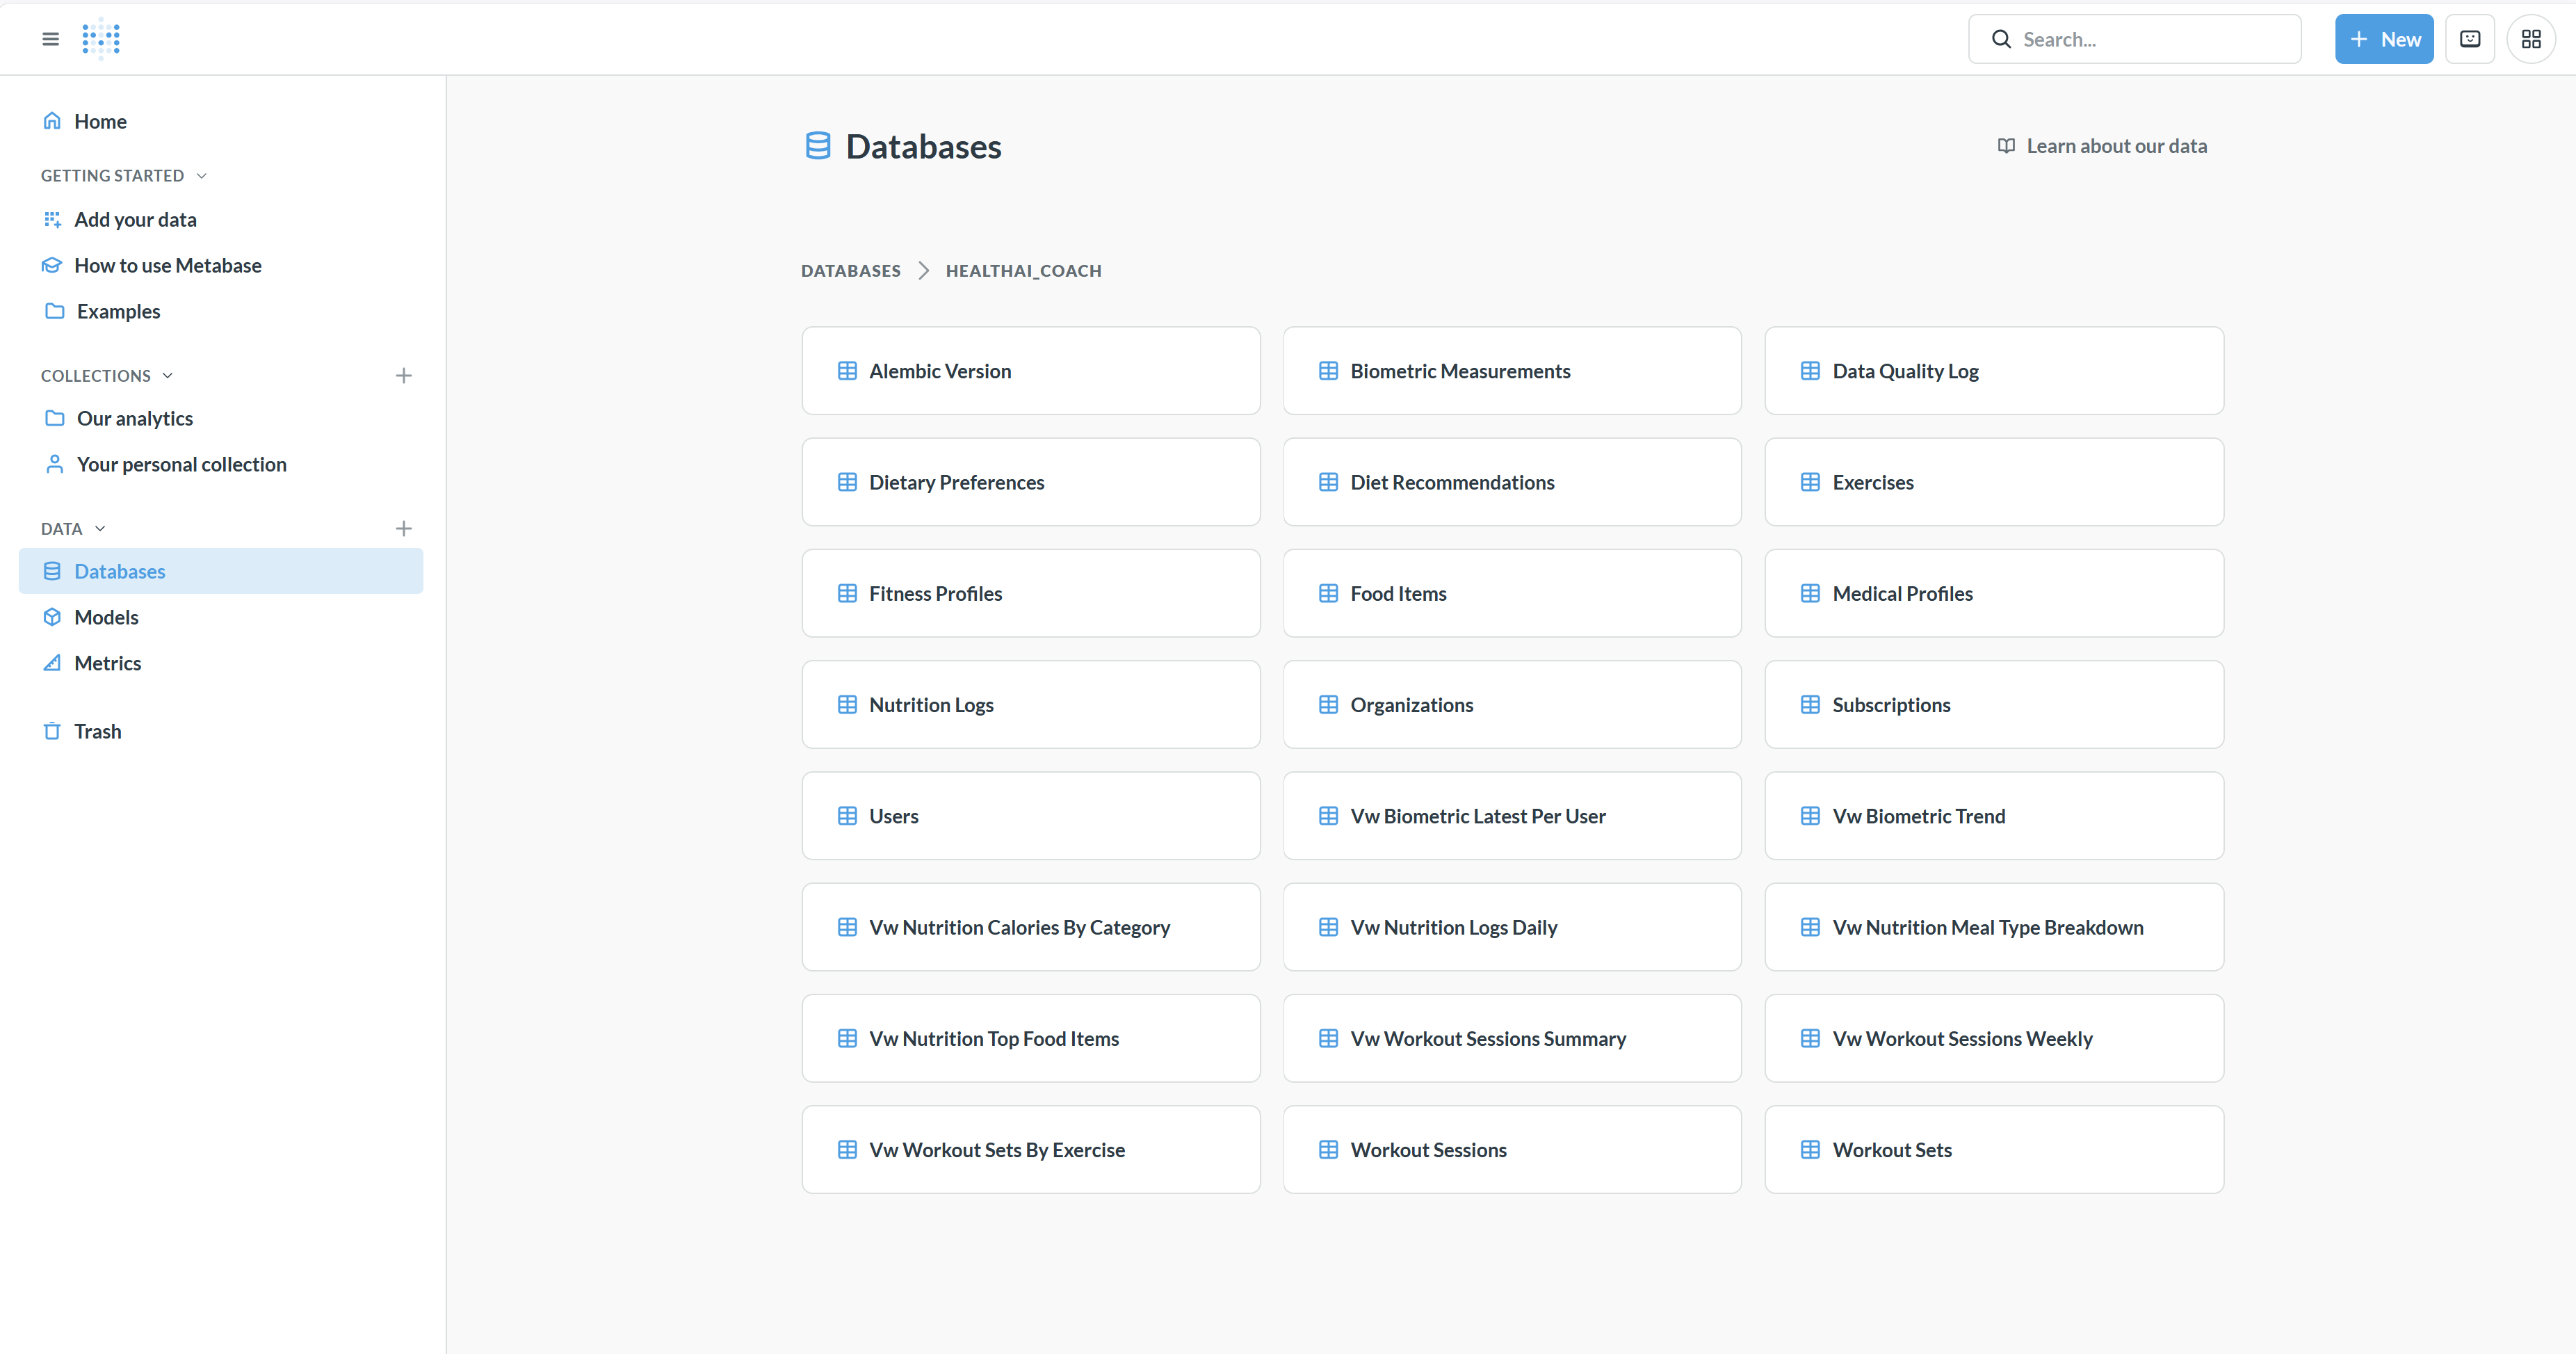
\includegraphics[width=\textwidth]{img/metabase_dashboard_db.png}
\caption{Metabase — schéma \texttt{healthai\_coach} exposé : les 14 tables et les vues KPI pré-construites.}
\label{fig:metabase-db}
\end{figure}

\begin{figure}[H]
\centering
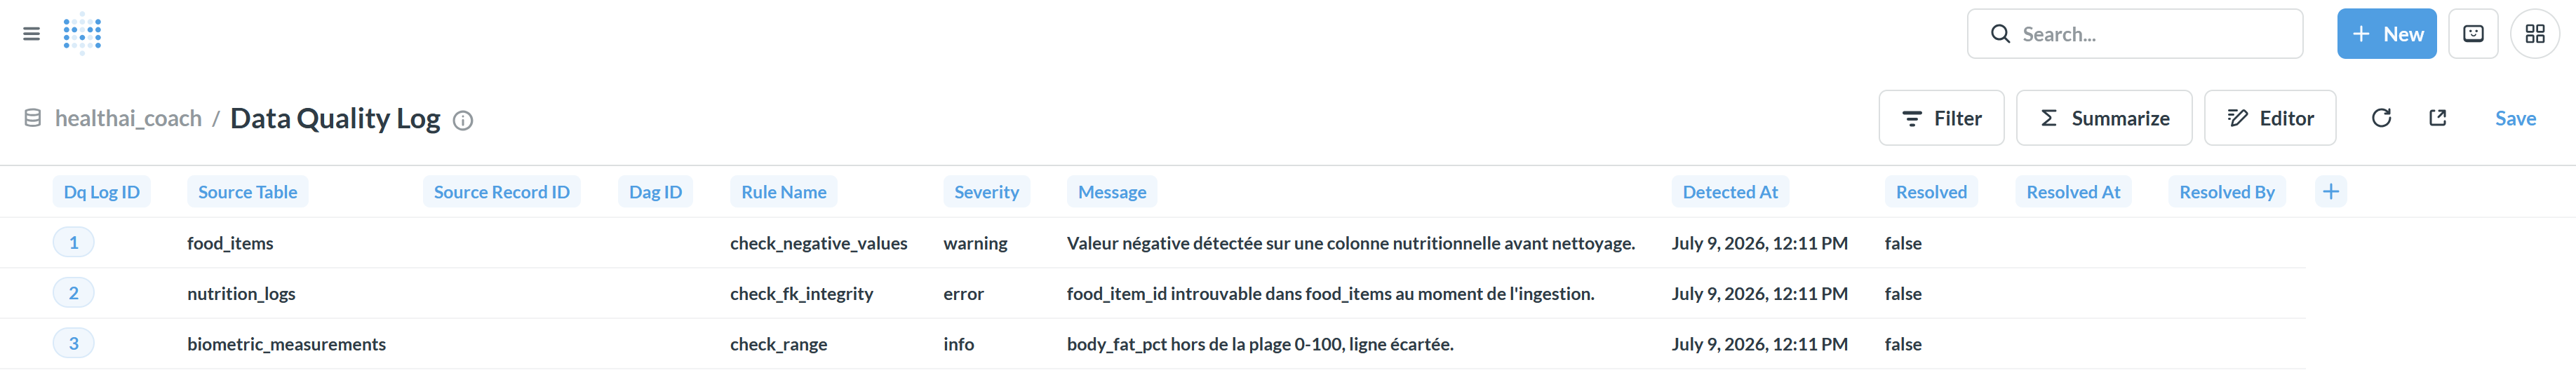
\includegraphics[width=\textwidth]{img/metabase_dashboard_qualite.png}
\caption{Metabase — consultation de \texttt{data\_quality\_log}, données réellement chargées en base.}
\label{fig:metabase-dql}
\end{figure}

Limitation assumée, propre au plan gratuit self-hosted : la personnalisation visuelle est restreinte à \texttt{Admin > Paramètres > Apparence} (nom de l'application, favicon, couleur primaire) ; le retrait du branding \og Powered by Metabase\fg{}, les palettes de couleurs de graphiques et les polices personnalisées sont réservés à l'offre Enterprise. Aucune méthode open source équivalente n'a été identifiée pour contourner cette restriction sans re-packager Metabase soi-même (hors périmètre). Décision : conserver le rendu par défaut plutôt que d'investir du temps sur ce point avant l'échéance.

% =============================================================================
\section{Dockerisation}
\label{sec:docker}
% =============================================================================

Objectif Sprint 6 : \texttt{docker compose up} $\rightarrow$ environnement fonctionnel en moins de 30 minutes, une seule commande. Huit services (\texttt{docker-compose.yml}) :

\begin{itemize}[leftmargin=1.4em]
  \item \textbf{postgres} (image officielle 16) — healthcheck \texttt{pg\_isready}, condition de démarrage pour les services suivants. Au tout premier démarrage (volume vierge), \texttt{database/init/*.sql} crée aussi les bases \texttt{metabase} et \texttt{airflow}, séparées de \texttt{healthai\_coach}.
  \item \textbf{db-init} — conteneur à usage unique (\texttt{service\_completed\_successfully}) : applique les migrations Alembic~\citep{alembic} puis peuple la base via \texttt{database/seed/seed\_data.py} (données fictives, dev/démo).
  \item \textbf{api} — démarre une fois \texttt{db-init} terminé avec succès, expose le port 8000 (\texttt{Dockerfile} fourni par l'équipe API, Rôle B).
  \item \textbf{admin\_interface} — démarre une fois \texttt{db-init} terminé avec succès, expose le port 7860.
  \item \textbf{metabase} — image officielle, même dépendance à \texttt{db-init}, expose le port 3000 ; connexion à PostgreSQL configurée une seule fois manuellement au premier lancement (Metabase n'expose pas d'API de pré-configuration).
  \item \textbf{airflow-init} — conteneur à usage unique : migre la base de métadonnées Airflow et crée le compte admin, via l'entrypoint officiel de l'image (\texttt{\_AIRFLOW\_DB\_UPGRADE}, \texttt{\_AIRFLOW\_WWW\_USER\_CREATE}).
  \item \textbf{airflow-webserver} / \textbf{airflow-scheduler} — démarrent une fois \texttt{airflow-init} terminé, exposent l'UI sur le port 8080. \texttt{LocalExecutor} + base \texttt{airflow} partagée sur le postgres du projet plutôt que le stack \texttt{CeleryExecutor}+Redis complet vu en formation (config commune factorisée via \texttt{x-airflow-common}, même principe que le patron officiel Airflow) : un DAG unique ne justifie pas plusieurs workers, et la machine de démo n'a pas la RAM pour 7 services Airflow en plus du reste de la stack applicative.
\end{itemize}

\paragraph{Point de vigilance — \texttt{db-init} ne deviendra pas le vrai pipeline ETL.} \texttt{db-init} exécute \texttt{seed\_data.py}, qui commence par un \texttt{TRUNCATE ... CASCADE} avant repeuplement : adapté au dev local et à la démo, mais incompatible avec le vrai pipeline (\texttt{etl/load}, Sprint 2), conçu pour upserter sans jamais tronquer et tourner de façon récurrente via le DAG Airflow \texttt{healthai\_etl\_pipeline} (Sprint 3). \textbf{Confirmé empiriquement, pas seulement théorique} : en testant le DAG (extraction réelle Kaggle/ExerciseDB, 2851 \texttt{users}, 645 \texttt{food\_items}, 404 \texttt{exercises} chargés), un simple redémarrage d'\texttt{admin\_interface} a redéclenché \texttt{db-init} qui a immédiatement tout effacé pour revenir aux 101/50/4 lignes de démo. \textbf{Résolu} : \texttt{db-init} respecte désormais la variable d'environnement \texttt{SEED\_DEMO\_DATA} (\texttt{.env}, défaut \texttt{true}) — une fois le vrai pipeline ETL en production, \texttt{SEED\_DEMO\_DATA=false} fait que \texttt{db-init} applique uniquement les migrations et les vues KPI, sans jamais tronquer de données réelles (cf. \texttt{docs/guide\_deploiement.md}).

\begin{figure}[H]
\centering
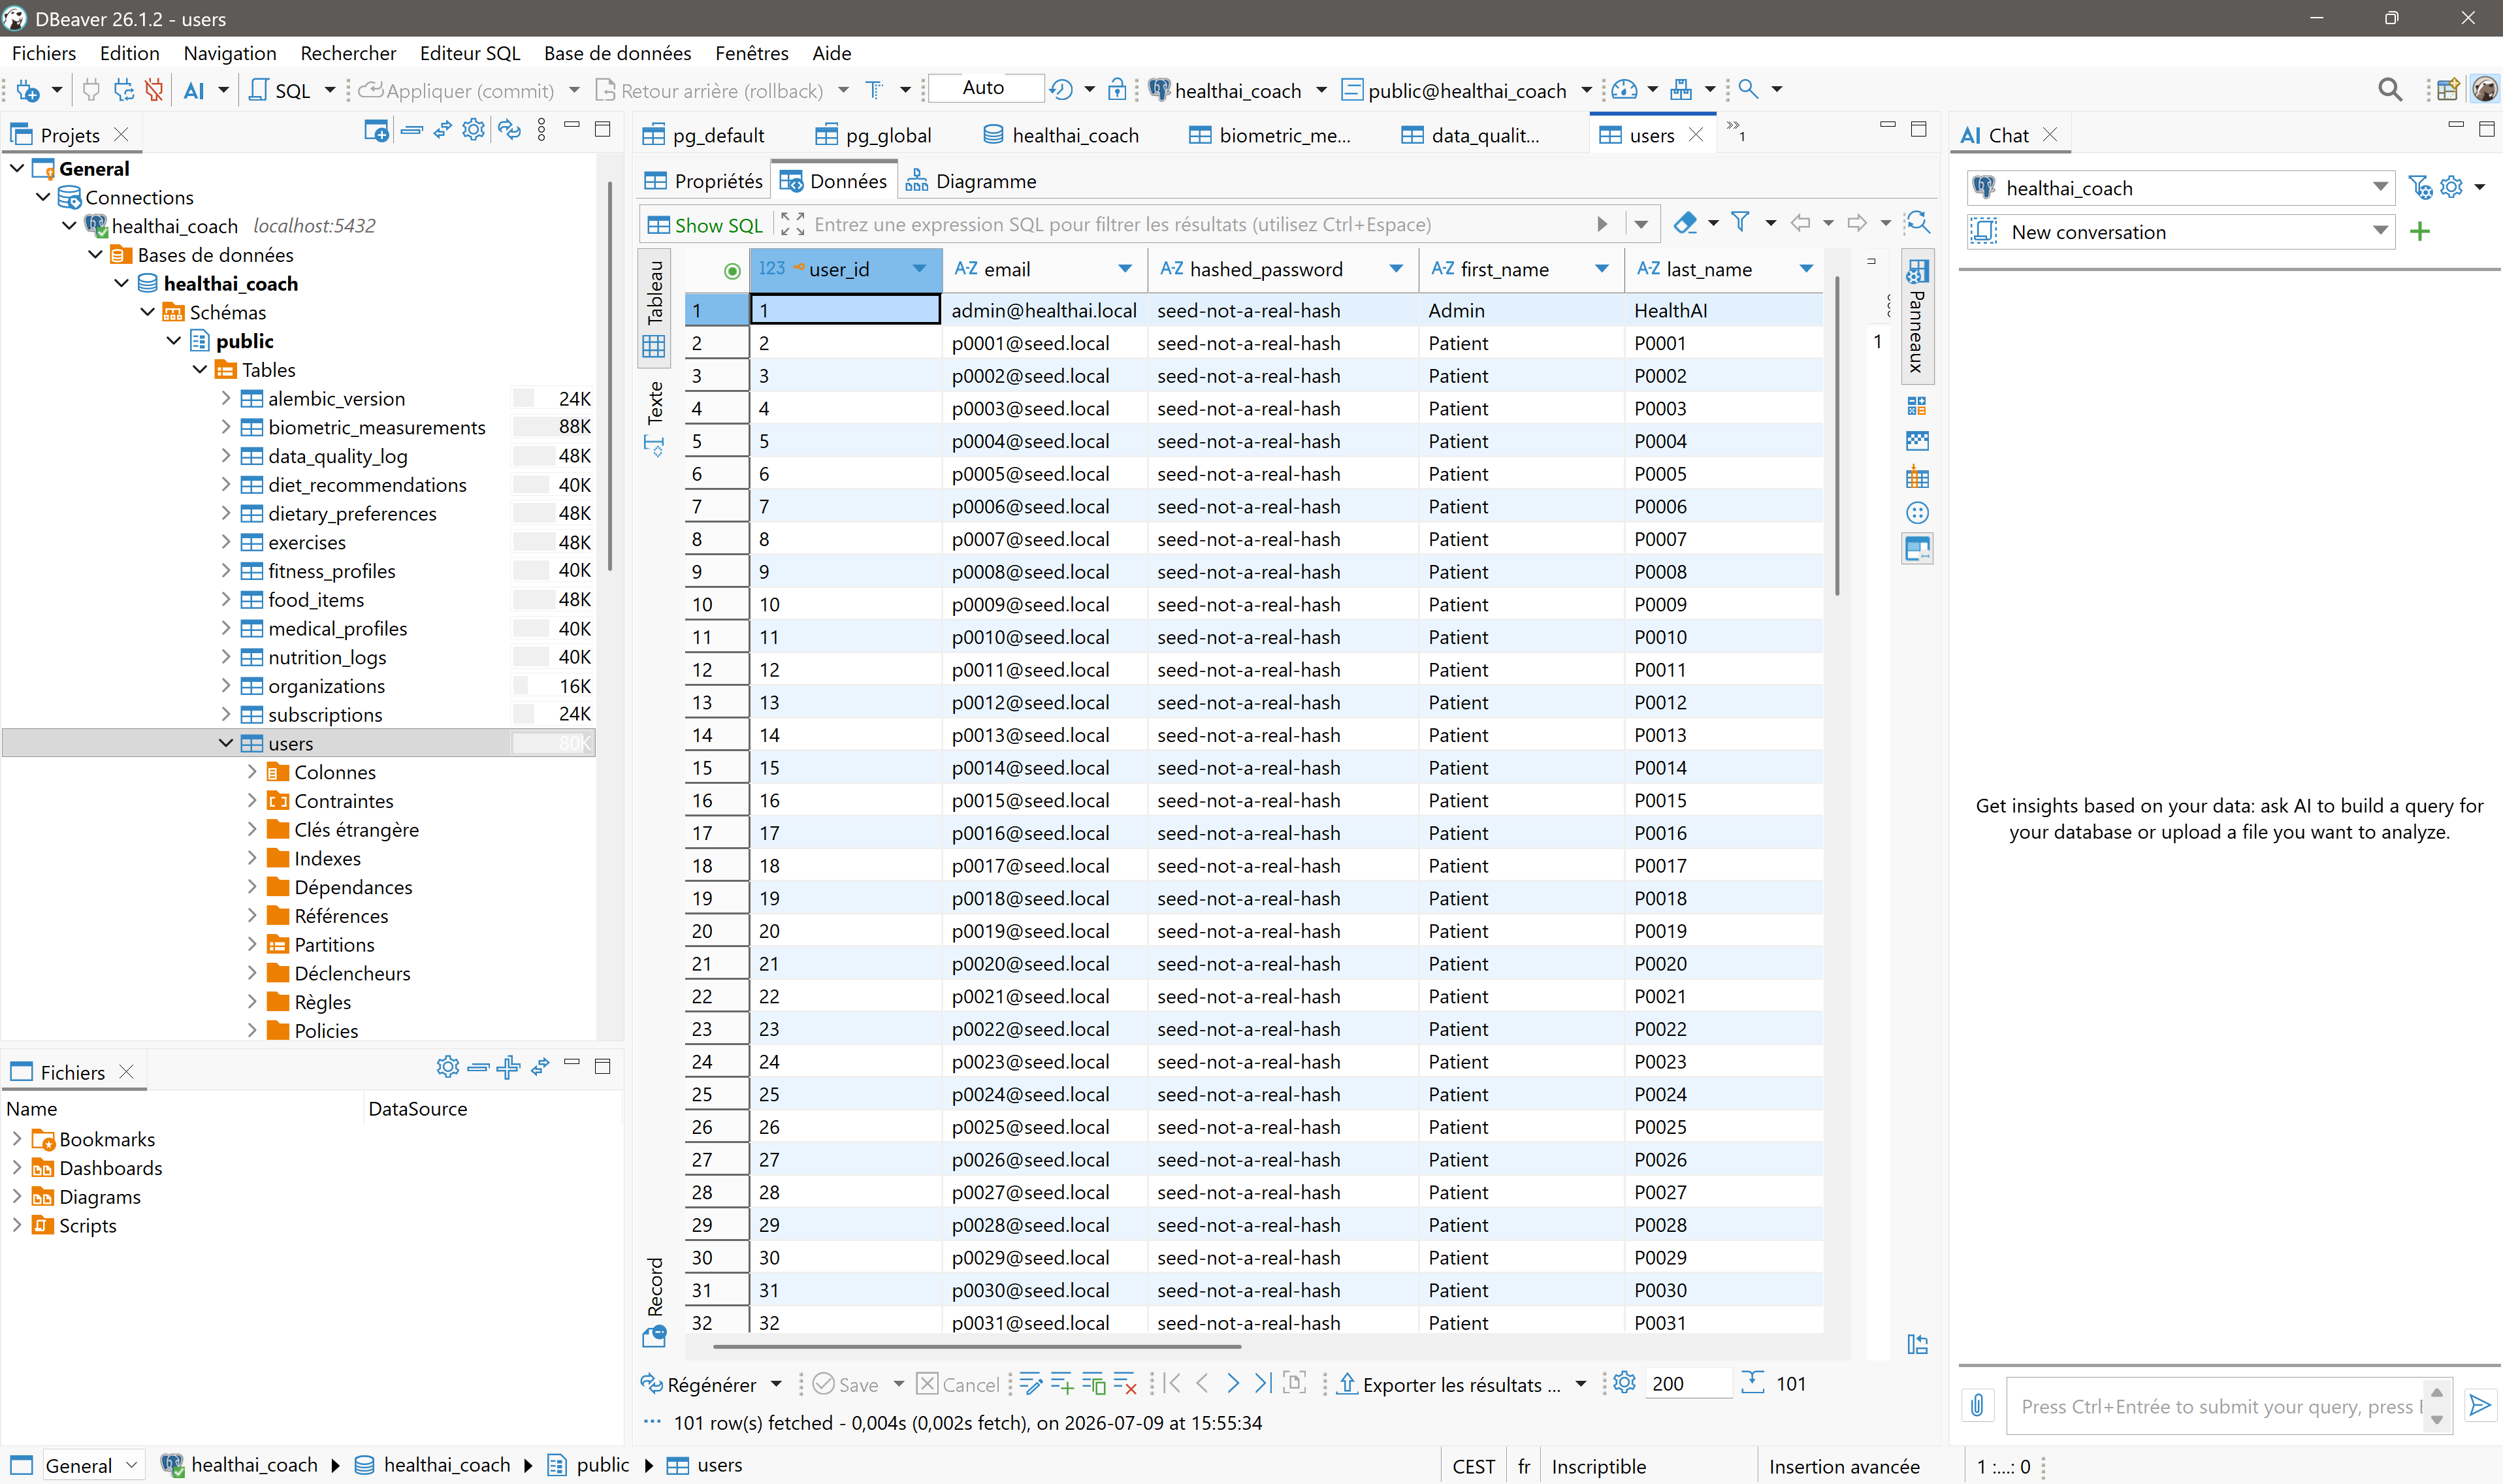
\includegraphics[width=\textwidth]{img/dbeaver_users_table.png}
\caption{Vérification du chargement réel des données (\texttt{users}, 101 lignes) via DBeaver connecté au conteneur \texttt{postgres}. On reconnaît la convention de seed dev/démo (\texttt{email} en \texttt{pXXXX@seed.local}, \texttt{hashed\_password = 'seed-not-a-real-hash'}) — à distinguer des vraies données produites par l'ETL une fois \texttt{load} en production (cf. point de vigilance ci-dessus).}
\label{fig:dbeaver-users}
\end{figure}

% =============================================================================
\section{Tests et CI/CD}
\label{sec:tests}
% =============================================================================

\subsection{Suite de tests}

\begin{table}[H]
\centering
\small
\begin{tabular}{@{}llr@{}}
\toprule
\textbf{Module} & \textbf{Périmètre} & \textbf{Fichiers} \\
\midrule
\texttt{tests/data\_quality/} & Schéma SQL : tables, FK, CHECK, cascades & 1 \\
\texttt{tests/admin\_interface/} & Interface admin : logique pure + DB réelle & 3 \\
\texttt{tests/api/} & Auth, users, organizations, subscriptions, contraintes & 7 \\
\texttt{tests/etl/} & Fonctions \texttt{transform} (mockées) + \texttt{quality/checks.py} (DB réelle) & 3 \\
\bottomrule
\end{tabular}
\caption{Suite de tests (141 tests au moment de la rédaction), \texttt{pytest}.}
\end{table}

Les tests \texttt{data\_quality}, \texttt{admin\_interface} et \texttt{etl/test\_quality\_checks.py} s'exécutent contre un PostgreSQL jetable (schéma reconstruit à chaque run depuis \texttt{ddl\_postgres.sql}) plutôt que des mocks, précisément parce que les contraintes \texttt{CHECK}/\texttt{FOREIGN KEY} sont une partie significative des règles métier du projet (cf. \S3.2) : un mock ne les vérifie pas. Cette différence de méthode s'est révélée concrète en cours de développement — une valeur \texttt{'Other'} (majuscule) produite par le module \texttt{transform} de l'ETL passait les 4 tests unitaires du module (entrées mockées) mais violait la contrainte \texttt{CHECK} réelle en base, détecté uniquement par insertion effective lors de la relecture de la PR correspondante.

\subsection{Pipeline CI}

GitHub Actions (\texttt{.github/workflows/ci.yml}), déclenché sur \texttt{pull\_request} et \texttt{push} vers \texttt{main}/\texttt{dev} : service PostgreSQL 16 éphémère, application des migrations Alembic (\texttt{alembic upgrade head}), puis \texttt{pytest tests/ -v}. Dépendances installées depuis deux fichiers consolidés (\texttt{database/migrations/requirements.txt} + \texttt{tests/requirements.txt}) plutôt que les \texttt{requirements.txt} propres à chaque module — point de vigilance pour la reproduction locale d'un échec CI : tester avec l'ensemble des \texttt{requirements.txt} du dépôt installés masque de vraies dépendances manquantes en CI (rencontré une fois en pratique, cf. \S8).

% =============================================================================
\section{Bilan et obstacles}
% =============================================================================

\subsection{Obstacles techniques rencontrés}

\begin{itemize}[leftmargin=1.4em]
  \item \textbf{Les tests mockés ne remplacent pas une vraie base} — une valeur \texttt{'Other'} produite par l'ETL passait 4/4 tests unitaires (entrées mockées) mais violait une contrainte \texttt{CHECK} réelle ; seule une insertion contre un PostgreSQL jetable l'a révélée (cf. \S3.2, \S\ref{sec:tests}). Décision prise en conséquence : les modules touchant au schéma sont désormais systématiquement re-testés contre une vraie base avant fusion, pas seulement via les tests unitaires du module.
  \item \textbf{Ma propre vérification manuelle de contraste RGAA était incomplète} — j'avais initialement validé le thème Gradio « à l'œil » sur quelques couleurs, en manquant les couleurs de texte \texttt{info=}/labels réellement utilisées. Un audit automatisé (\texttt{axe-core}) a révélé l'erreur (2,56:1 au lieu de 4,5:1 requis) — corrigé depuis (cf. \S\ref{sec:admin-interface}). À retenir : l'automatisation prime sur la relecture manuelle pour ce type de vérification.
  \item \textbf{Reproduction fidèle de la CI} — un premier échec CI (\texttt{ModuleNotFoundError: gradio}) n'était pas reproductible en local parce que l'environnement de test local avait plus de dépendances installées que la CI réelle (tous les \texttt{requirements.txt} du dépôt, alors que la CI n'en installe que deux). Depuis, toute validation de correctif reproduit exactement la séquence de commandes CI dans un environnement vierge avant d'être considérée acquise.
  \item \textbf{\texttt{db-init} vs pipeline ETL réel, confirmé en conditions réelles} — le risque théorique identifié dès la PR \#44 (\texttt{TRUNCATE} de \texttt{db-init} vs upsert jamais destructeur du vrai pipeline) s'est concrètement produit en testant le DAG Airflow : un redémarrage anodin d'\texttt{admin\_interface} a effacé des données réelles fraîchement chargées (cf. \S\ref{sec:docker}). La bascule (retirer \texttt{seed\_data.py} de \texttt{db-init} ou la conditionner) reste à trancher, mais n'est plus un risque abstrait pour la suite du projet.
  \item \textbf{Conflit de version SQLAlchemy avec Airflow} — Airflow 2.10.5 exige \texttt{SQLAlchemy<2.0} en interne, alors que le reste du projet (y compris \texttt{etl/}) utilise \texttt{2.0.51} depuis le début. Installer les dépendances ETL dans le même environnement Python que Airflow les aurait fait cohabiter et aurait risqué de casser le webserver/scheduler — détecté via les avertissements \texttt{pip} au moment du build de l'image, avant tout déploiement. Résolu par un venv Python isolé à l'intérieur de l'image Airflow, les tâches du DAG l'invoquant en sous-processus plutôt que d'importer \texttt{etl/} dans le process Airflow.
\end{itemize}

\subsection{Points positifs}

\begin{itemize}[leftmargin=1.4em]
  \item Contraintes d'intégrité (\texttt{CHECK}, \texttt{FOREIGN KEY}, index uniques partiels) portées directement par PostgreSQL plutôt que dans le code applicatif : les règles métier survivent à n'importe quel point d'entrée (API, ETL, script ad hoc), pas seulement à un chemin de code particulier.
  \item Schéma auto-documenté (\texttt{COMMENT ON TABLE/COLUMN}) : les conventions non triviales (clé d'upsert, distinction cholestérol alimentaire/sanguin, etc.) sont lisibles depuis la base elle-même, pas seulement dans un document externe qui peut diverger du schéma réel.
  \item Convention d'idempotence (\texttt{UNIQUE(source, external\_id)}, \texttt{Faker.seed()} déterministe) définie une fois puis reprise à l'identique par l'équipe ETL sur chaque nouvelle source, et par l'équipe API pour le pattern d'historisation (\texttt{diet\_recommendations} $\rightarrow$ \texttt{workout\_plans}/\texttt{nutrition\_plans}, cf. PR \#52).
  \item Discipline de revue systématique (checkout isolé, tests rejoués contre PostgreSQL frais, jamais de confiance aveugle dans un diff ou un « les tests passent ») qui a détecté plusieurs bugs réels avant fusion plutôt qu'en production.
\end{itemize}

% =============================================================================
\section{Conclusion}
% =============================================================================

Le backend HealthAI Coach couvre, à date de rédaction, un schéma PostgreSQL de 16 tables avec ses migrations Alembic, une API REST authentifiée (utilisateurs, journaux nutrition/activité, abonnements, routes IA prêtes pour un microservice pas encore déployé), un pipeline ETL complet et orchestré (extraction, transformation, chargement idempotent et contrôle qualité enchaînés par un DAG Airflow testé de bout en bout contre des données réelles), une interface d'administration de la qualité des données auditée RGAA, un dashboard Metabase, et une conteneurisation \texttt{docker compose} (sept services) permettant de démarrer l'ensemble en une seule commande.

Le principal facteur limitant a été le temps disponible dans le cadre de cette formation, pas une difficulté technique bloquante : le microservice IA n'est qu'esquissé (stub côté API), l'incompatibilité entre \texttt{db-init} et le vrai pipeline ETL est identifiée et documentée mais pas encore tranchée, et certaines limitations d'accessibilité du composant \texttt{Dataframe} de Gradio ne sont pas corrigibles sans reconstruire le composant lui-même. Le choix a été fait de prioriser la robustesse de ce qui est livré (contraintes en base, tests contre une vraie base de données, CI reproductible, pipeline ETL vérifié en conditions réelles plutôt que supposé fonctionnel) plutôt que de couvrir l'intégralité du périmètre imaginé au démarrage — un compromis assumé plutôt qu'un oubli.

% =============================================================================
\begin{thebibliography}{99}

\bibitem{kaggle_nutrition} Adil Shamim, \emph{Daily Food and Nutrition Dataset}. Kaggle, 2024. \url{https://www.kaggle.com/datasets/adilshamim8/daily-food-and-nutrition-dataset}

\bibitem{kaggle_diet} Ziya, \emph{Diet Recommendations Dataset}. Kaggle, 2024. \url{https://www.kaggle.com/datasets/ziya07/diet-recommendations-dataset}

\bibitem{kaggle_gym} Vala Khorasani, \emph{Gym Members Exercise Dataset}. Kaggle, 2023. \url{https://www.kaggle.com/datasets/valakhorasani/gym-members-exercise-dataset}

\bibitem{kaggle_fitness} Nadeem Ajeed, \emph{Fitness Tracker Dataset}. Kaggle, 2024. \url{https://www.kaggle.com/datasets/nadeemajeedch/fitness-tracker-dataset}

\bibitem{exercisedb} \emph{ExerciseDB API — documentation}. \url{https://oss.exercisedb.dev}

\bibitem{postgresql} PostgreSQL Global Development Group, \emph{PostgreSQL Documentation}. \url{https://www.postgresql.org/docs/}

\bibitem{alembic} Mike Bayer, \emph{Alembic Documentation}. \url{https://alembic.sqlalchemy.org}

\bibitem{sqlalchemy} Mike Bayer, \emph{SQLAlchemy Documentation}. \url{https://docs.sqlalchemy.org}

\bibitem{airflow} Apache Software Foundation, \emph{Apache Airflow Documentation}. \url{https://airflow.apache.org/docs/}

\bibitem{fastapi} Sebastián Ramírez, \emph{FastAPI Documentation}. \url{https://fastapi.tiangolo.com}

\bibitem{pydantic} Pydantic, \emph{Pydantic Documentation}. \url{https://docs.pydantic.dev}

\bibitem{faker} Faker contributors, \emph{Faker Documentation}. \url{https://faker.readthedocs.io}

\bibitem{gradio} Gradio, \emph{Gradio Documentation}. \url{https://www.gradio.app/docs}

\bibitem{metabase} Metabase, \emph{Metabase Documentation}. \url{https://www.metabase.com/docs/latest/}

\bibitem{axecore} Deque Systems, \emph{axe-core — Accessibility Engine}. \url{https://github.com/dequelabs/axe-core}

\bibitem{rgaa} DINUM, \emph{Référentiel Général d'Amélioration de l'Accessibilité (RGAA) 4.1}. \url{https://accessibilite.numerique.gouv.fr/}

\end{thebibliography}

% =============================================================================
\appendix
\section{Extrait du schéma SQL — tables principales}
% =============================================================================

Extrait de \texttt{database/schema/ddl\_postgres.sql} illustrant les patterns récurrents du schéma : contraintes \texttt{CHECK} sur domaine de valeurs fermé, clé d'idempotence \texttt{UNIQUE}, contrainte de cohérence multi-colonnes, et FK optionnelle avec \texttt{ON DELETE SET NULL}.

\begin{lstlisting}[style=sql]
CREATE TABLE users (
    user_id         SERIAL PRIMARY KEY,
    email           VARCHAR(255) NOT NULL UNIQUE,
    hashed_password VARCHAR(255) NOT NULL,
    first_name      VARCHAR(100) NOT NULL,
    last_name       VARCHAR(100) NOT NULL,
    date_of_birth   DATE,
    sex             VARCHAR(10) CHECK (sex IN ('F', 'M', 'other')),
    is_admin        BOOLEAN NOT NULL DEFAULT FALSE,
    created_at      TIMESTAMPTZ NOT NULL DEFAULT now(),
    updated_at      TIMESTAMPTZ NOT NULL DEFAULT now()
);

CREATE TABLE food_items (
    food_item_id    SERIAL PRIMARY KEY,
    external_id     VARCHAR(100),
    source          VARCHAR(50) NOT NULL,
    name            VARCHAR(255) NOT NULL,
    calories_kcal   NUMERIC(7,2) NOT NULL CHECK (calories_kcal >= 0),
    ingested_at     TIMESTAMPTZ NOT NULL DEFAULT now(),
    UNIQUE (source, external_id)  -- cle d'upsert idempotent (cf. S3.2)
);

CREATE TABLE data_quality_log (
    dq_log_id         BIGSERIAL PRIMARY KEY,
    source_table      VARCHAR(100) NOT NULL,
    rule_name         VARCHAR(150) NOT NULL,
    severity          VARCHAR(20) NOT NULL
                      CHECK (severity IN ('info', 'warning', 'error', 'critical')),
    message           TEXT NOT NULL,
    detected_at       TIMESTAMPTZ NOT NULL DEFAULT now(),
    resolved          BOOLEAN NOT NULL DEFAULT FALSE,
    resolved_at       TIMESTAMPTZ,
    resolved_by       INTEGER,
    CONSTRAINT fk_data_quality_log_resolved_by
        FOREIGN KEY (resolved_by) REFERENCES users(user_id) ON DELETE SET NULL,
    CONSTRAINT chk_data_quality_log_resolution_consistency
        CHECK (resolved = TRUE OR (resolved_at IS NULL AND resolved_by IS NULL))
);
\end{lstlisting}

\end{document}
